\documentclass[a4paper,12pt]{book}

% Paquetes necesarios
\usepackage[utf8]{inputenc}   % Codificación de caracteres
\usepackage[spanish]{babel}   % Idioma español
\usepackage[T1]{fontenc}      % Codificación de fuentes
\usepackage{amsmath, amssymb} % Símbolos matemáticos
\usepackage{graphicx}         % Inclusión de gráficos
\usepackage{cite}             % Gestión de citas
\usepackage{hyperref}         % Enlaces y referencias
\usepackage{geometry}         % Configuración de márgenes
\usepackage{fancyhdr}         % Encabezados y pies de página
\usepackage{titlesec}         % Formato de títulos
\usepackage{booktabs}         % Tablas profesionales
\usepackage{caption}          % Personalización de leyendas
\usepackage{enumitem}         % Personalización de listas
\usepackage{float}
\usepackage{tcolorbox}
\usepackage[table]{xcolor} % Paquete para colores en tablas
\usepackage{colortbl}       % Complemento para colorear celdas específicas
\usepackage{multirow}       % Combinar celdas en tablas
\usepackage{makecell}       % Combinar celdas en tablas
\usepackage{enumitem}
\usepackage{amsmath}
\usepackage{eurosym}
\usepackage{tikz}
\usepackage{listings}
\usepackage{color}
\usepackage{float}
\usepackage{pdfpages}
\usepackage{subfigure}
% Configuración de márgenes
\geometry{left=3cm, right=3cm, top=2.5cm, bottom=2.5cm}

% Configuración de encabezados y pies de página
% \setlength{\headheight}{14.49998pt}
\pagestyle{fancy}
\fancyhf{}
\fancyhead[L]{Universidad de Granada}
\fancyhead[L]{\nouppercase{\leftmark}}

% \fancyhead[C]{Escuela Técnica Superior de Ingenierías Informática}
\fancyhead[R]{Fundamentos de Base de Datos}
\fancyfoot[L]{\rule[0pt]{\textwidth}{0.2pt}\\Ismael Sallami Moreno}
\fancyfoot[C]{\rule[0pt]{\textwidth}{0.2pt}\\\thepage}
\fancyfoot[R]{\rule[0pt]{\textwidth}{0.2pt}\\\today}
\renewcommand{\sectionmark}[1]{\markboth{#1}{}} % Configura \leftmark para que solo muestre la sección


% Formato de títulos
\titleformat{\section}{\large\bfseries}{\thesection.}{0.5em}{}
\titleformat{\subsection}{\normalsize\bfseries}{\thesubsection.}{0.5em}{}

% Datos del documento
\title{\textbf{Temario Inteligencia Artificial}}
\author{
    Ismael Sallami Moreno \\
    \texttt{ism350zsallami@correo.ugr.es}
}
\date{
    \vspace{1cm}
    \begin{tabular}{rl}
        \textbf{Asignatura:} & Fundamentos de Base de Datos \\
        \textbf{Tema:} & Teoría \\
        \textbf{Fecha:} & \today
    \end{tabular}
}

% Comando para definir código en línea que se muestra en cursiva y no se sale del PDF
\newcommand{\inlinecode}[1]{\texttt{\textit{#1}}}


\begin{document}

% Portada
\begin{titlepage}
    \begin{center}
        % \vspace*{1cm}
        
        % \Huge
        % \textbf{Práctica Contabilidad Financiera II}
        \Huge \textbf{FBD - Relación de Ejercicios Tema 3: Modelo Racional} 
        % \vspace{0.5cm}
        % \LARGE
        % \textbf{Ismael Sallami Moreno}\\
        % \LARGE
        % \texttt{ism350zsallami@correo.ugr.es}
        % \LARGE
        % \url{https://github.com/Ismael-Sallami}
        
        % \vfill
        
        % \Large
        % \textbf{Universidad de Granada}
        
        \vspace{0.8cm}
        
        \begin{tikzpicture}[remember picture, overlay]
            \node[opacity=0.2] at (current page.center) {
\includegraphics[width=\paperwidth,height=\paperheight]{portada.jpg}};
            \node[align=center] at (current page.center) {
                
                \vspace{0.5cm}
                \LARGE \textbf{Ismael Sallami Moreno} \\
                \LARGE \texttt{ism350zsallami@correo.ugr.es} \\
                %\LARGE \url{https://ismael-sallami.github.io/} \\
                %\LARGE \url{https://elblogdeismael.github.io/} \\
                \vspace{2cm}
                \Large \textbf{Universidad de Granada} \\
                \vspace{0.8cm}
                % \Large \textbf{2025}
            };
        \end{tikzpicture}
        \vfill
        
        \Large
        \textbf{2025}
        
    \end{center}
\end{titlepage}
\newpage


%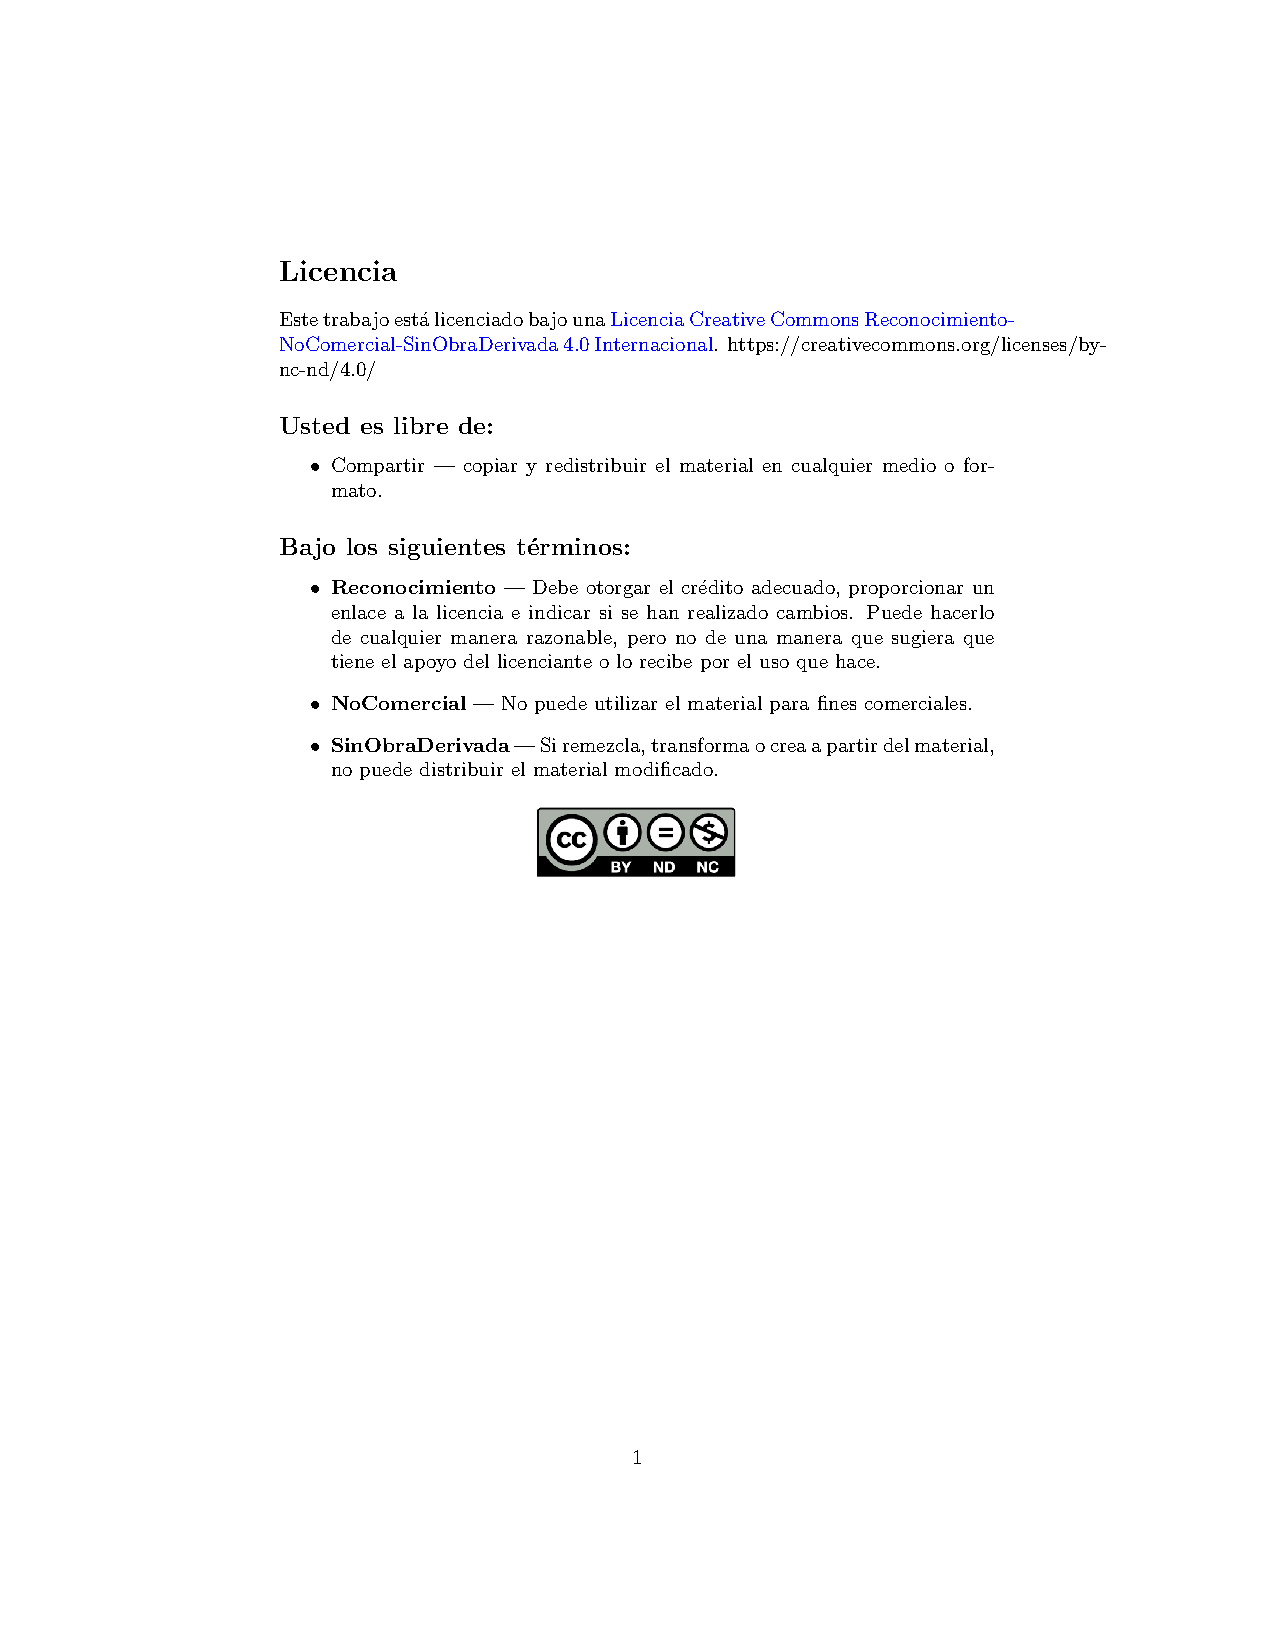
\includepdf[pages=-]{../../../../licencia.pdf}
% Tabla de contenidos
\tableofcontents
\newpage

\chapter{Modelo de Datos: Modelo Racional}

\section{Definición}

Previamente, debemos de llevar a cabo un análisis de los datos y de esta manera obtenemos el esquema conceptual y lógico de la BD. En este tema entre la siguiente fase de \textit{Diseño}, dando como resultado el modelo lógico. Este se trata de uno ya implementado, por eso se dice que es un modelo implementable. 

En cuanto al proceso de transformación, distinguimos:

\begin{enumerate}
    \item Mundo real 
    \item Datos operativos
    \item Esquema conceptual
\end{enumerate}

En esta etapa se introduce lo que conocemos como \textit{tablas}. En la última fase llevamos a cabo la implementación de esa tabla mediante un lenguaje.

Definición: Mecanismo formal para representar y manipular la información con la que voy a trabajar. Debe de constar de datos, operaciones y reglas de integridad.

La necesidad de usar el modelo de datos son:
\begin{itemize}
    \item Se usan lenguajes de definición de datos.
    \item Es de muy bajo nivel.
    \item Se necesitan niveles superior para su abstracción.
\end{itemize}

El objetivo que se tiene es establecer que representen los datos y que los describan de una forma entendible y manipulable. Según ANSI distinguimos tres niveles:
\begin{itemize}
    \item Externo
    \item Conceptual
    \item Interno
\end{itemize}

En cuanto a la clasificación:
\begin{itemize}
    \item Basados en registros.
    \item Basados en objetos.
    \item Físico.
\end{itemize}

Los dos primeros son de nivel externo y conceptual, mientras que el último es de nivel interno.

\section{Modelo Relacional}

La información se organiza en tablas: 

\begin{enumerate}
    \item La estructura de almacenamiento son las tablas.
    \item Integridad.
    \item Consulta y Manipulación.
\end{enumerate}

Esta tabla es a nivel lógico, en cuanto al nivel físico depende de varias estructuras, como son las listas enlazadas,...

Elementos a conocer:
\begin{itemize}
    \item Atributo.
    \item Dominio: rango de valores que puede tomar (enteros, letras,...)
    \item Relación: Se conoce como cualquier subconjunto del producto cartesiano $D_1 \times D_2 \times ... D_n$. En este caso a relación se refiere a la tabla. Se denota como $R(A_1..A_n)$. De esta manera conseguimos todos los valores que pueden tomar y de aquí sacamos los datos (solo a nivel teórico).
    \item Tupla: filas de la tabla.
    \item Cardinalidad de una relación: número de tuplas.
    \item Esquema de una relación R: Atributos de la relación junto a su dominio.
    \item Grado de una relación: Número de atributos. Aunque se supone que es invariable, esto depende ya que se puede modificar.
    \item Instancia de una relación: datos que tengo en un determinado momento.
    \item Esquema de la BD: colección de esquemas de relaciones junto con las restricciones de integridad.
    \item Instancia o estado de una BD: colección de instancias de relaciones que verifican las condiciones de integridad.
    \item BD relaciones: instancia de la BD junto con su esquema.
\end{itemize}

\subsubsection*{Condición de Normalización}

\begin{itemize}
    \item Todos los valores de los atributos de una relación son atómicos\footnote{No se pueden dividir más}.
    \item Valor atómico es un valor no estructurado.
    \item Cuando una relación cumple la condición de normalización se dice que está en Primera Forma Normal.
\end{itemize}

\subsubsection*{Consecuencias}

\begin{itemize}
    \item No hay valores tipo conjunto.
    \item No hay valores tipo registro.
    \item No hay valores tipo tablas.
\end{itemize}

\subsubsection*{Problema}

Todas las representaciones son extensivas, no se puede representar información del tipo “el valor del atributo asignaturas de un alumno es: FBD, ALG, LD”.


\subsubsection*{Consecuencias de la definición}

\begin{itemize}
    \item No hay tuplas duplicadas:
    \begin{itemize}
        \item Por la definición conjuntista de relación.
    \end{itemize}
    \item No hay orden en las filas ni en los atributos:
    \begin{itemize}
        \item Al no estar ordenados ni los atributos ni las filas (conjuntos) el acceso es por nombre de atributo y valor.
    \end{itemize}
    \item Varias instancias representan la misma relación.
\end{itemize}

\begin{table}[h!]
\centering
\begin{tabular}{|c|c|c|c|c|}
\hline
A & B & C & D & E \\ \hline
a1 & b1 & c1 & d1 & e1 \\ \hline
a1 & b2 & c2 & d2 & e1 \\ \hline
a2 & b1 & c3 & d3 & e1 \\ \hline
a2 & b1 & c4 & d3 & e1 \\ \hline
a3 & b2 & c5 & d1 & e1 \\ \hline
\end{tabular}
\end{table}

\begin{table}[h!]
\centering
\begin{tabular}{|c|c|c|c|c|}
\hline
A & B & C & D & E \\ \hline
a2 & b1 & c4 & d3 & e1 \\ \hline
a2 & b1 & c3 & d3 & e1 \\ \hline
a1 & b2 & c2 & d2 & e1 \\ \hline
a3 & b2 & c5 & d1 & e1 \\ \hline
a1 & b1 & c1 & d1 & e1 \\ \hline
\end{tabular}
\end{table}

En cuanto a las representaciones podemos distinguir:
\begin{itemize}
    \item Representación física: Archivos, registros y campos.
    \item Representación intuitiva: Tabla, filas y columnas.
    \item Modelo matemático: Relación, tuplas y atributos.
\end{itemize}

\section{El modelo de datos relacional. ED. Integridad}
\subsection{La estructura de datos relacional}

\subsection*{Notación a utilizar}
\begin{itemize}
    \item Relación: R, S, T....
    \item Atributos: A, B, ...
    \item Esquema de relación: R[A1, A2, ..., An]
    \item Instancia de relación R: r
    \item Tuplas de una instancia: x1, x2, ..., $\in$ r
    \item Valor de un atributo Ai en una tupla xj: xj[Ai] ó Aij
\end{itemize}

\subsection*{Valores nulos}
\begin{itemize}
    \item Algunas veces no se conoce el valor de un atributo para una determinada tupla. En esos casos a ese atributo de esa tupla se le asigna un valor nulo (NULL).
    \item Un valor nulo puede ser:
    \begin{itemize}
        \item Un valor desconocido.
        \item Un atributo no aplicable.
    \end{itemize}
    \item En cualquier caso, ese valor es un valor más de todos los dominios de la base de datos.
\end{itemize}

\subsection{Restricciones o reglas de integridad}

\begin{itemize}
    \item Son condiciones para preservar la semántica de una base de datos.
    \item Específicas del problema:
    \begin{itemize}
        \item $0 \leq \text{edad} \leq 100$
        \item $\text{créditos} > 0$
        \item $\text{carácter} \in \{\text{'troncal', 'obligatoria', 'optativa', ...}\}$
    \end{itemize}
    \item Propias del papel de los atributos en el esquema:
    \begin{itemize}
        \item $\text{imparte.NRP} \in \text{profesor.NRP}$ (un profesor inexistente no puede impartir una asignatura)
        \item $\text{cod\_asig} \neq \text{nulo}$ (siempre debe conocerse el código de una asignatura)
    \end{itemize}
\end{itemize}

\subsection*{Superclaves y claves (candidatas y primarias)}
\begin{itemize}
    \item Superclave: Cualquier conjunto de atributos que identifica unívocamente a cada tupla de una relación.
    \item Clave de una relación: superclave minimal.
    \item Por ejemplo, en la relación Asignaturas:
    \begin{itemize}
        \item El conjunto de atributos \{Cod\_Asig, Nombre\} identifica unívocamente cada tupla.
        \item Sin embargo, no es minimal y no puede considerarse como una clave.
        \item Cod\_Asig por sí sola, es una clave.
    \end{itemize}
\end{itemize}

\begin{itemize}
    \item En una relación dada puede que más de un conjunto de atributos puedan ser elegidos como clave. Estos conjuntos de atributos se llaman claves candidatas.
    \item Cuando hay más de una clave candidata, hay que seleccionar una como principal. Esta clave recibe el nombre de clave primaria de la tabla.
    \item Criterio de selección: Tamaño, significado, \textbf{capacidad para recordarla}\footnote{Ejemplo de ello, es cuando vas a secretaría a preguntar por algo, donde te preguntan por tu DNI, en vez de Nº de expediente.}, fusión con otras tablas, etc.
\end{itemize}

\subsubsection*{Clave candidata y primaria (definición formal)}

\begin{itemize}
    \item Sea R[A1, A2, ..., An], CC $\subseteq \{A1, A2, ..., An\}$ se denomina clave candidata si y solo si:
        \begin{itemize}
            \item \textbf{Unicidad}: $\forall r$ instancia de R y $\forall t1, t2 \in r$ con $t1 \neq t2 \Rightarrow t1[CC] \neq t2[CC]$\footnote{No puede coincidir dos tuplas distintas.}
            \item \textbf{Minimalidad}: No existe CC' $\subseteq$ CC que verifique la unicidad.
        \end{itemize}
        \item Una clave candidata es un atributo o conjunto de atributos que identifican a cada tupla en la relación y que, además, no existe un subconjunto de ellos que también identifiquen a cada tupla de la relación.
        \item Una clave primaria es una clave candidata elegida por el diseñador.
        \item Si CC verifica la unicidad pero no la minimalidad se denomina superclave.
        \item Completamos la notación para describir una relación, subrayando los atributos que forman su clave primaria etiquetándolos con CP. Si existen otras claves candidatas también se subrayan etiquetando el subrayado con CC:
        \begin{itemize}
            \item Socio (\underline{\#Socio\textsubscript{CP}}, \underline{DNI\textsubscript{CC}}, Nombre, Dirección)\footnote{En este caso estamos denotando como se referencia en la práctica.}
        \end{itemize}
\end{itemize}

\subsubsection*{Claves externas}

\begin{itemize}
    \item Conjunto de atributos en una relación que es una clave en otra (o incluso en la misma) relación.
    \item Podemos ver una clave externa como un conjunto de atributos de una relación cuyos valores en las tuplas deben coincidir con los valores de la clave primaria de las tuplas de la otra relación.
\end{itemize}

\subsubsection*{Claves externas}

\begin{itemize}
    \item Consideramos una relación R (relación que referencia) y un subconjunto de atributos de su esquema CE (clave externa); y una relación S (relación referenciada) cuya clave primaria CP coincide con CE.
    \item Si CE es una clave externa de R que referencia a CP en S, entonces: $\forall t \in r, \exists t' \in s$ tal que $t[CE] = t'[CP]$, donde $r$ y $s$ son las instancias de R y S en la base de datos.
    \item Eventualmente, R y S pueden ser la misma relación.
\end{itemize}

\begin{itemize}
    \item Ejemplo: Imparte (NRP, Cod\_Asig) referencia a Profesor (NRP).
\end{itemize}

\subsubsection*{Dominio activo}

\begin{itemize}
    \item Subconjunto de valores del dominio de un atributo de una relación que está presente en la instancia de la relación\footnote{Es decir, en un momento dado.}.
    \item Dada una relación R, su instancia r y un atributo A de R, el dominio activo de A es el siguiente conjunto:
    \[
    \{a \mid \exists t \in r \text{ tal que } t[A] = a\}
    \]
    \item Podemos extender el concepto de dominio activo a un conjunto de atributos.
    \item Dada una relación R, su instancia r y un subconjunto de atributos CA de R, el dominio activo de CA es el siguiente conjunto:
    \[
    \{(a_1, a_2, \ldots, a_n) \mid \exists t \in r \text{ tal que } t[CA] = (a_1, a_2, \ldots, a_n)\}
    \]
    \item Las claves externas establecen relaciones de inclusión entre los dominios activos de la clave externa y la clave referenciada.
\end{itemize}

\begin{itemize}
    \item Puede haber más de una clave externa en una relación.
    \item Puede haber una clave externa a la clave primaria de la propia relación\footnote{No puede haber  dos claves en la misma sección que se llamen igual, por lo que si en una relacion nos encontramos con dos DNI, debemos de denotar uno de manera distinta, o bien usar una notación distinta.}.
    \item El resultado de que haya CE con una misma relación es el hecho de la \textit{fusión de tablas}.
\end{itemize}

\subsection*{Conceptos generales}
\begin{itemize}
    \item Condiciones de integridad:
    \begin{itemize}
        \item Normas que mantienen la corrección semántica de una base de datos.
    \end{itemize}
    \item Nos centramos en la integridad genérica: depende del papel que juegue un atributo en el diseño de la tabla:
    \begin{itemize}
        \item Son metarreglas: generan reglas de integridad aplicadas a una base de datos concreta.
        \item Existen la integridad de entidad y la integridad referencial.
    \end{itemize}
\end{itemize}

\subsubsection*{Integridad de entidad}
\begin{itemize}
    \item No se debe permitir que una entidad sea representada en la base de datos si no se tiene una \textbf{información completa} de los atributos que son clave primaria de la entidad.
    \item Un atributo que forma parte de la clave primaria de una tupla en una relación, \textbf{no puede tener un valor nulo}\footnote{Esto define la integridad de la tabla.}.
\end{itemize}

\subsubsection*{Integridad referencial}
\begin{itemize}
    \item Una base de datos en la que \textbf{todos los valores no nulos de una clave externa referencian valores reales de la clave referenciada} en la otra relación, cumple la regla de integridad referencial. Si esto se cumple, estamos cumpliendo con la regla de \textit{integridad referencial}.
    \item Si una relación incluye una clave externa conectada a una clave primaria, el valor de la clave externa debe ser, o bien igual a un valor ya existente en el dominio activo de la clave primaria, o bien completamente nulo (si la semántica lo permite).
    \item La integridad referencial mantiene las conexiones en las bases de datos relacionales.
\end{itemize}

\subsection*{Restricciones del SGBD}

EL SGBD debe encargarse de mantener las siguientes restricciones:
\begin{itemize}
    \item La unicidad de la clave primaria y de las claves candidatas:
    \begin{itemize}
        \item Frente a operaciones de inserción y actualización, el SGBD debe rechazar los valores introducidos que sean iguales a los presentes en la BD para los atributos que el diseñador ha definido como clave primaria y como claves candidatas.
    \end{itemize}
    \item La integridad de identidad:
    \begin{itemize}
        \item Frente a operaciones de inserción y actualización, el SGBD debe rechazar las modificaciones que asignen un valor NULO a algún atributo de la clave primaria.
    \end{itemize}
\end{itemize}

\begin{itemize}
    \item La integridad referencial:
    \begin{itemize}
        \item En inserciones:
        \begin{itemize}
            \item Rechazar la tupla insertada si el valor de la clave externa no concuerda en la relación referenciada para alguna tupla en el valor su clave primaria, es decir, si no es nulo o bien no existe.
            \item Si el valor para la clave externa es NULO y el diseño no lo permite, habrá que \textit{rechazar} también esa inserción.
        \end{itemize}
        \item En borrados:
        \begin{itemize}
            \item Si se borra la clave primaria en la relación referenciada, el diseñador puede establecer en el SGBD una de las siguientes alternativas de actuación:
            \begin{itemize}
                \item Rechazar el borrado de la tupla.
                \item Eliminar en cadena todas las tuplas que la referencian.
                \item Poner valor nulo en la clave externa de todas esas tuplas.
            \end{itemize}
        \end{itemize}
        \item En actualizaciones:
        \begin{itemize}
            \item Si se actualiza la clave externa, actuar con el nuevo valor actualizado como en el caso de inserción.
            \item Si se actualiza la clave primaria de la relación referenciada y el antiguo valor estaba referenciado en alguna relación, actuar como en el caso de borrado.
        \end{itemize}
    \end{itemize}
\end{itemize}

\section{Otros modelos de datos}

\subsection{Modelo jerárquico}

Fue el primero en implementarse físicamente:
\begin{itemize}
    \item Nivel externo: aplicaciones Cobol o lenguaje del sistema.
    \item No había interactividad:
    \begin{itemize}
        \item Carecía de un lenguaje de consulta.
    \end{itemize}
    \item Estructura de datos básica:
    \begin{itemize}
        \item Árbol:
        \begin{itemize}
            \item Registro maestro: raíz.
            \item Registros secundarios: dependen de los anteriores.
        \end{itemize}
    \end{itemize}
    \begin{itemize}
        \item La BD es una colección de instancias de árboles.
        \item Esta estructura plasma de forma muy directa:
        \begin{itemize}
            \item Relaciones muchos a uno.
            \item Relaciones uno a uno.
        \end{itemize}
        \item Para relaciones muchos a muchos:
        \begin{itemize}
            \item Hay que duplicar toda la información sobre las entidades involucradas.
        \end{itemize}
    \end{itemize}
\end{itemize} 



\newpage
% Referencias
\begin{thebibliography}{99}
\bibitem{Referencia1}
Ismael Sallami Moreno, \textbf{Estudiante del Doble Grado en Ingeniería Informática + ADE}, Universidad de Granada, 2025.
% \bibitem{Referencia2}
% Autor(es), \emph{Título del libro}, Editorial, año.

% \bibitem{Referencia3}
% Autor(es), \emph{Título del documento}, Nombre de la Conferencia, páginas, año.
\end{thebibliography}

\end{document}
